\section{Webes keretrendszerek}
	\paragraph{}
	A keretrendszerek napjainkban felkapott rendszerek lettek a felhasználók között. Ezek a rendszerek sokoldalúak, robusztusak és hatékonyak. A különböző alkalmazások fejlesztéséhez az ilyen jellegű rendszerek segítségével csak a magasabb szintű funkcionalitások elvégzésére kell koncentrálni. Erre az a magyarázat, hogy a keretrendszer gondoskodik az alacsonyabb funkcionalitásokról, amelyek már rengeteg tesztelt kódot tartalmaznak, így mi ezeket a funkcionalitásokat nem kell külön megírjuk és leteszteljük, hogy helyes-e a megírt kód. Számos előnyt lehet felsorolni, hogy miért jó ha használjuk ezeket a rendszereket.\cite{frameworks}
	\begin{itemize}
		\item Elősegíti a tervezési minták megfelelő kialakítását.
		\item Biztonságosabb kódolás.
		\item A redundáns kód elkerülése.
		\item Következetes kódfejlesztés kevesebb hibával.
		\item Megkönnyíti a kód tesztelését és a hibakeresést is.
		\item Az alkalmazás fejlesztéséhez szükséges idő lecsökken.
	\end{itemize}
	\paragraph{}
	 \ref{fig:vueang} ábrán megtekínthetjük, hogy a 2016-os évtől a 2019-es évig a webes keretrendszerek egy része az érdeklődési és az elégedettségi szint alapján a használatosságuk hogyan változik.
	
	\begin{figure}
		\centering
		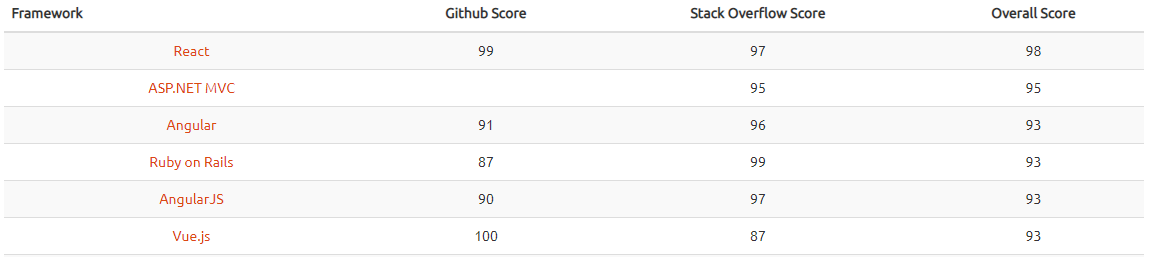
\includegraphics[scale=0.6]{figures/images/vueang.png}
		\caption{Webes keretrendszerek használatossága érdeklődési és elégedettségi szint alapján \cite{vueanginterest}}
		\label{fig:vueang}
	\end{figure}

	\subsection{Angular}
	\paragraph{}
	Az Angulart \cite{wohlgethan2018supportingweb} 2008-ban kezdték el fejleszteni a Google munkatársai. A fejlesztés JavaScriptben történt. Abban az időben a webhelyek többsége többoldalas alkalmazás megközelítésén alapult. Ennek viszont a teljesítménye az idő elteltével romlani kezdett mivel befolyásoló tényező lett az internet kapcsolat és a szerver reakció képessége is. Ezért létre hozódott az egy oldalas alkalmazások megközelítése ami abban segít, hogy a több oldalas weboldalak csupán egy oldalon jelennek meg. Az Angular volt az egy oldalas alkalmazások első kerete. Az egyik fő előnye, hogy a felhasználók egyszerű struktúrával kell dolgozzanak. Megtanulják az Angular sajátos felépítését ezáltal gyorsan és optimálisabban tudnak benne fejleszteni. Az sem elhanyagolható, hogy a fejlesztők egy részletes és egyértelmű dokumentációval szolgáltak a felhasználóknak. Egy TypeScript nyelv amely hasznos és könnyen használható. A TypeScript nyelvek nagyon elterjedtek lettek. 
	
	\subsection{Vue.js}
	\paragraph{}
	A Vue.js (röviden: Vue) \cite{wohlgethan2018supportingweb} tekinthető a legújabb keretrendszernek. Hasonlít az Angularhoz. Mindkéttő TypeScript típusú. Használható kisebb, egyszerűbb projekteknél és egy komplexebb egy oldalas alkalmazás elkészítésénél is. Fő érdeme a skálázhatóság. Különlegessége, hogy egy nyílt forráskódú közösség fejlesztette ki, nem pedig egy nagyobb vállalat. Komponens alapú keretrendszer amely azt jelenti, hogy komponenseket különböztetünk és jelenítünk meg. Egy komponensen belül tudunk írni HTML, CSS és Script elemeket is. A megjelenítés egy oldalon történik ezért szükséges használni a útválasztást(rout).
	
	\subsection{Angular vs Vue.js}
	\paragraph{}
	Mindkét keretrendszernek megvannak az előnyei \ref{tab:table1} táblázat és a hátrányai is \ref{tab:table2} táblázat. 
	\begin{table}[H]
	\begin{footnotesize}
		\begin{center}
			\caption{Előnyök Angular és Vue.js között \cite{vuevsang} }
			\label{tab:table1}
			\begin{tabular}{p{2cm}|p{6cm}|p{6cm}}
				\textbf{Sorszám} & \textbf{Angular} & \textbf{Vue.js}\\
				\hline
				1 & TypeScript használata & TypeScript használata, részletes dokumentáció\\
				\hline
				2 & Részletes dokumentációval rendelkezik & Egy oldalas alkalmazások készítése \\
				\hline
				3 & Gyorsítja a fejlesztést & Könnyű integráció a meglévő struktúrákba \\
				\hline
				4 & & Kihasználja virtuális DOM előnyeit \\
				\hline
				5 & & Sebessége és rugalmassága optimális \\
			\end{tabular}
		\end{center}
	\end{footnotesize}
	\end{table}

	\begin{table}[H]
	\begin{footnotesize}
		\begin{center}
			\caption{Hátrányok Angular és Vue.js között \cite{vuevsang}}
			\label{tab:table2}
			\begin{tabular}{p{2cm}|p{6cm}|p{6cm}} 
				\textbf{Sorszám} & \textbf{Angular} & \textbf{Vue.js}\\
				\hline
				1 & Számos különféle struktúrát kínál, nehezíti a tanulást & Kevesebb erőforrást kínál\\
				\hline
				2 & Lassabb teljesítmény mert működik a reális DOM &  \\
			\end{tabular}
		\end{center}
	\end{footnotesize}
	\end{table}

	\subsection{NodeJs}
	\paragraph{} 
	A NodeJs \cite{js2016node} egy olyan szoftver platform, amely a Chrome V8 JavaScript futási idején épül fel. Fontos tulajdonsága, hogy skálázható ezért is sokan használják. Eseményvezérelt, nem blokkoló I/O modellt használ, amely könnyűvé és hatékonnyá teszi a valós idejű alkalmazásokhoz, amelyek elosztott rendszeren futnak át. Használatos mivel aszinkron és a tanulási görbéje is helyén van. A fejlesztők hatalmas köre már évek óta ismeri a JavaScriptet és az aszinkron programozást. Legtöbb esetben a NodeJs használatakor adatbázisnak NoSQL adatbázisokat választanak.
	
	\subsection{Spring Boot}
	\paragraph{}
	A Spring Boot \cite{jovanovic2017java} célja a Spring alkalmazás fejlesztés egyszerűsítése. Megtalálhatóak benne a következő tulajdonságok:
	\begin{itemize}
		\item Automatikus konfigurációk - Az alkalmazások Springként való működése érdekében.
		\item Indítófüggőségek - Biztosítja a felhasználóknak a szükséges függőségek(dependency) beimportálását. Ilyen lehet a Maven, Hibernate validátor, adatbázis eléréseket stb.
		\item Parancssori tolmács.
		\item Működtetés - A console-ba megjelennek az alkalmazás működésével kapcsolatos információk. Ilyen információ lehet a hiba, az elvégzett művelet stb.
	\end{itemize}
	
	\paragraph{}
	Radikálisan gyorsabb és széles körben hozzáférhető, érthető Spring fejlesztést nyújt. Számos funkciót kínál: beágyazott szervereket, metrikákat, ellenőrzéseket, külső konfigurációkat. Saját struktúrával rendelkezik és nem tesz különbséget az adatbázisok között. A JAVA nyelvet használja.
	
	\subsection{NodeJs vs Spring Boot}
	\paragraph{}
	NodeJs a következő különlegességeket tartalmazza \cite{nodejsspring}:
	\begin{itemize}
		\item A NodeJS alkalmazások fejlesztésének elindítása könnyű.
		\item Az agilis fejlesztési módszertant követi, amely alkalmas a nagyon skálázható alkalmazásfejlesztési szolgáltatásokra.
		\item Nagy projekteknél gyorsabban működik mint a Java.
		\item Hatalmas erőforrás-készlet könyvtárakkal rendelkezik
	\end{itemize}
	
	\paragraph{}
	Spring Boot a következő különlegességeket tartalmazza \cite{nodejsspring}:
	\begin{itemize}
		\item Egyszerű, minden eszköz és operációs rendszer támogatja.
		\item Beépített nyelvbiztonsági funkciókkal rendelkezik, amelyeket a Java Compiler beágyaz.
		\item Robusztus kódot alkalmaz.
		\item Integrációs képesség jó.
		\item Az alkalmazások egyszerűen építhetőek fel.
		\item Beágyazott HTTP-kiszolgálókat, például Jetty, Tomcat használ és egyszerűen teszteli a webes alkalmazásokkal.
	\end{itemize}
	
	\paragraph{}
	A fent leírtakat figyelembe véve utána néztem, hogy a NodeJs és a Spring Boot milyen érdekeltségi szinttel rendelkezik az emberek körében. Ezt megfigyelhetjük a  \ref{nodespring}. \cite{nodejsspring1} Mindkét keretrendszert inkább backend fejlesztésére használják.
	
	\begin{figure}
		\centering
		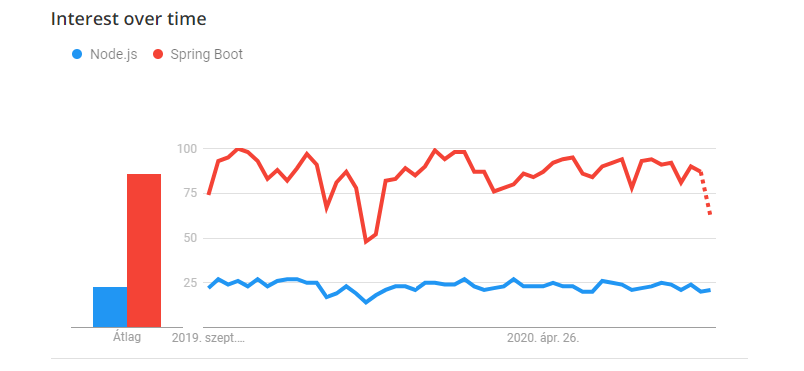
\includegraphics[scale=0.9]{figures/images/nodespring.png}
		\caption{NodeJS és SpringBoot érdekeltségi szintje}
		\label{nodespring}
	\end{figure}